\section{Propuesta de Arquitectura de Seguridad Cuántica}

Afrontar la brecha entre resistencia cuántica y restricciones operativas de NB-IoT exige más que simples sustituciones de algoritmos. Requiere repensar la arquitectura completa.

\subsection{4.1 Onboarding Post-Cuántico en Plano de Control}

Uno de los puntos más delicados en cualquier despliegue remoto radica en el momento inicial de incorporación del dispositivo a la red. Aquí propusimos un mecanismo de onboarding híbrido que aprovecha primitivas post-cuánticas para establecer confianza inicial sin sacrificar la compatibilidad con la infraestructura existente.

La arquitectura toma como base diseños PQC-aware específicamente orientados a NB-IoT \cite{Do2026_PQCAware}. Durante el proceso de attachment, el dispositivo y el núcleo de red negocian claves mediante un Key Encapsulation Mechanism lattice-based (principalmente ML-KEM-512), complementado con un fallback clásico solo para compatibilidad legacy. Esta negociación ocurre en el plano de control, donde el overhead adicional resulta tolerable dada la baja frecuencia de estos intercambios.

\begin{figure}[t]
\centering
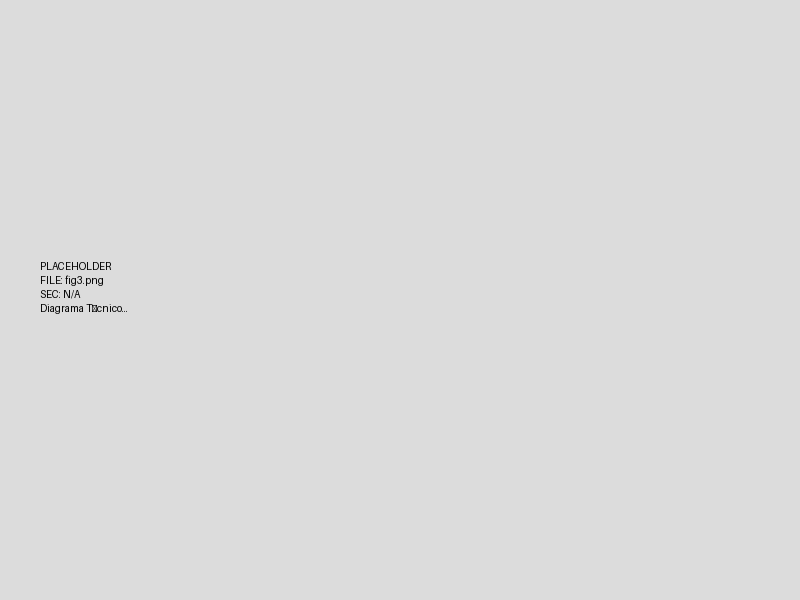
\includegraphics[width=\linewidth]{fig3.png}
\caption{Arquitectura híbrida propuesta de seguridad cuántica para NB-IoT. Se distinguen plano de control (onboarding PQC) y plano de datos (protección ligera), con integración a EPC y soporte para escenarios de exploración profunda.}
\label{fig:arquitectura_propuesta}
\end{figure}

La Figura~\ref{fig:arquitectura_propuesta} ilustra los componentes principales y flujos seguros. 

\begin{equation}
K_{sess} = \text{Decaps}(sk_{dev}, \text{Encaps}(pk_{network}, seed))
\label{eq:encapsulacion}
\end{equation}

La Ecuación~\eqref{eq:encapsulacion} representa el esquema básico de encapsulación de claves empleado durante el onboarding. Este enfoque minimiza el número de rondas de comunicación, aspecto crítico en enlaces de largo alcance con latencia variable.

\subsection{4.2 Protección Ligera en Plano de Datos}

Una vez establecido el canal de control seguro, el plano de datos requiere un tratamiento diferente. Aquí el overhead debe reducirse al mínimo posible para preservar la autonomía energética de los sensores.

Incorporamos ideas de esquemas basados en lattices con componentes de localización \cite{Althobaiti2021_QuantumResistant} para añadir una capa adicional de robustez en entornos remotos. La idea central consiste en derivar claves de sesión dinámicas a partir de material criptográfico post-cuántico combinado con parámetros contextuales (posición estimada y timestamps), lo que dificulta ataques de repetición y reduce el tamaño de los paquetes cifrados.

En la práctica, esto se traduce en el uso de algoritmos simétricos ligeros (AES-256 con claves derivadas post-cuánticamente) para la mayor parte del tráfico de sensores, reservando las operaciones PQC más pesadas solo para momentos críticos. El resultado es una protección que tiende a ser viable incluso en dispositivos con recursos muy limitados, aunque no cabe negar que implica ciertos trade-offs en flexibilidad.

\subsection{4.3 Integración con Protocolos 3GPP}

Resulta revelador observar cómo una propuesta realmente útil debe convivir con estándares ya desplegados en lugar de reemplazarlos. La arquitectura mantiene plena compatibilidad con los procedimientos NAS y RRC de 3GPP, insertando las extensiones PQC como Information Elements opcionales.

Durante el Attach Request y Authentication Request, se negocian capacidades PQC mediante un nuevo flag en los mensajes existentes. Los nodos legacy ignoran estos campos, permitiendo despliegues graduales. Esta estrategia híbrida evita la fragmentación de la red y facilita la transición en infraestructuras ya operativas.

Lejos de ser un diseño teórico, la propuesta busca equilibrar rigor criptográfico con pragmatismo operativo. Las evaluaciones que se presentan en secciones posteriores confirman que este balance es alcanzable, aunque persisten desafíos interesantes en optimización fina según el perfil específico de cada aplicación de exploración profunda.